\documentclass[12pt]{article}

% Language setting
% Replace `english' with e.g. `pathspanish' to change the document language
\usepackage[english]{babel}

% Set page size and margins
% Replace `letterpaper' with`a4paper' for UK/EU standard size
\usepackage[a4paper,top=2cm,bottom=2cm,left=3cm,right=3cm,marginparwidth=1.75cm]{geometry}

% Useful packages
\usepackage{amsmath}
\usepackage{graphicx}
\usepackage[colorlinks=true, allcolors=black]{hyperref}


%title
\title{\underline{AutoPylot}}
\date{January 2022 - May 2022}

\author{%
    \\
    Maxime Ellerbach \\
    Mickael Bobovitch \\
    Alexandre Girold \\
    Maxime Gay \\ \\
    Group: Autonomobile 
    }

\begin{document}
\maketitle
\newpage

\tableofcontents
\newpage

\section{Introduction}
Autonomous vehicles and more specifically self driving cars have grasp the attention of many people for good or ill. In this spirit, we have decided with the Autonomobile team to create our first ever project, Autopolyt.

What is Autopylot's goal ? 
Drive itself on a track and win races. It may, at first glance seem very simple but not everything is at it seems. Yet we will try to make it as easy to undestand as possible, without omiting crutial information. To achieve our goal, we need to solve many other problems. Those problems can be separate into two distinct groups. 
    
The first one would be the software part. Indeed in this project we will need to learn and acquire certain skills, from teamwork to coding in different languages. With those newly acquired skills we will be able to bring machine learning to our car to make it drive itself. This leads use directly to our second part, the more tangible one : hardware. Indeed, as we will progress in our work, we will need to see the results of our work in real life condition. This means implementing our code to a functioning car which will be able to race on a track.

This project will lead by a team of four young developers, Maxime Ellerbach, Mickael Bobovich, Maxime Gay and Alexandre Girold. In this project work will be divided equally amongst all of us, sometimes we will have to work together to achieve our very tight time frame. 

\subsection{Project nature}
Autonomous cars will likely dominate our roads in a relatively close future.
With this project, we aim to have a first approach to such a complex problem by participating in the DiyRobocars competition.
We will be using a 1:10 scale radio controlled car modified to integrate onboard computer such as a raspberry pi and some sensors.

\subsection{State of the art}
In this section, we will try to see what was previously made in this sector of industry.
It would not be realistic to compare our 1:10 project to real sized cars such as Tesla's, simply because in a racing environnement,
we don't need to deal with such an amount of safety: pedestrian detection, emergency braking, speed limit detection and other.
So we will only see miniature autonomous racing framework that we would likely race against.\\

The most known is called "DonkeyCar", created by Will Roscoe and Adam Conway in early of 2017. Most of the models trained with DonkeyCar are behavior cloning models, meaning models that tries to replicate the behavior of a driver. This methods uses a big amount of images (input) associated to steering angles and throttle (output), it requires the user to drive the car (collect data) prior to training the model: no examples means no training. The lack of training data often leads to the car leaving the track.\\

One other framework worth looking at is one created by Nvidia called "JetRacer" released in 2019. It uses a different approach from DonkeyCar where the user annotates the images by hand by clicking on where the car should go. The model used is similar to what DonkeyCar uses meaning a Convolutional Neural Network with one input (the image) and two outputs, one for the steering angle and one for the throttle to apply. \\

Both of those framework are written in python and use packages such as Tensorflow and OpenCV, we will also use them in our project.

\section{Objectives}

\subsection{Final objectives}
Our main objective is to make our car race against other cars and win the race !
This will require multiple intermediate milestones:
\begin{itemize}
\item Being able to send scripted controls to the motor and servo.
\item Being able to drive the car manually using a controller.
\item Develop a way to gather images and annotations and store them in a stuctured way, for example sorted by date.
\item Process those data before feeding them to the neural network.
\item Being able to train a convolutional neural network using those data.
\item Construct a telemetry web app.
\item Tweak the architecture and the parameters of the chosen model to acheive the best results.
\item Test in real life the model.
\item Race against other !
\end{itemize}
Once all of that is done, we will start our optional objectives that will enable better racing and better understanding of the car's environnement.

\subsection{Optional objectives}
To be able to go faster and increase the reliability of our car's driving, we will need to add some features to our project. \\

One good feature would be to have a model that takes into account the speed of the car. As we all know on a real car, we don't steer the same way when going at 10km/h and going at 90km/h. This input extension could bring more stability to our model.
To go faster, it would also be great to be able to differenciate turns from straight lines and even braking zone before the turn. \\

One of the challenges racing implies is overtaking. Overtaking is a very complex manoeuver. First we obviously need to be faster than the car ahead, we could assure that by detecting the successive positions of the car ahead on the image. If the car is getting closer, it's Y coordinate will come closer to the bottom of our image. Also, we cannot overtake if we have no room for that, that means we have to detect a gap on the left or the right of the car before initiating the overtake. Once we decided on what part of track we will overtake, we still need to get ahead of the opponent's car. We could acheive that by forcing the model to drive on the left or right part of the track for a given amount of time.

% paragraphe mika 
\subsection{Motivations}
Why this project ? 

This project is something that we deeply care about. Being able to work on an self driving car does sound like a dream to most of us. Yet thanks to Reda Dehak, we made that dream come true. Being able to work on this project means we will be able to learn valuable skills for our futur life. Being able to work on this project is also a way to prove ourselves, that with enough work anything is achivable.

Our goal is not to make the new tesla model W but be a part of this constant progress in autonomus vehicules. We also want to see how far we can take this project and what we will have achieved by the end of the school year. With this idea in mind we have set ourself some goals, for example winning a race. This project is not a common one but that is exactly what pushes us to make it work not matter the cost. We are also proud to be able to represent Epita for the races. 


% The concept of an autonomous car is nothing new. Indeed, many achievements have been made. Both real and miniature size cars exist but their implementation is different. In fact, there is a huge gap of technologies between. We want to reduce this gap. We want to succeed in implementing the safety and stability of cars in productions like Tesla. Our goal is not to make a miniature Tesla, but to take back the safety elements. It is common for miniaturized cars to slip off the tracks for lack of environmental detection. We want to use the latter method for entourage detection. So far, a large part of the implementations uses line detections. We want to go beyond the comfort zone and use a different and innovative method that is based on AI. We want to take the best of what is out there and explore possibilities to make self-driving miniature cars that are reliable and capable of racing other vehicles. Until now miniaturized cars did not take into account other vehicles. They are considered the only vehicle on the track and the overtaking principle was not implemented. We will try to beat this challenge. Indeed, this is something unusual. We want to make a real leap forward in this area and not just replicate what is out there. To simplify our task, we will be content to run races. The recognition of panels and pedestrians is too complex for us. Large-scale racing and artificial intelligence are a little exploited field. This is what push us to create something new. We will be happy to represent EPITA at the next cars races and win for our School. We would be very proud of it.

\section{Technical specifications}

\subsection{Hardware}
On the hardware side, we already have a working car containing:
\begin{itemize}
\item A RaspberryPi 4. It is used for heavy computations like image processing, model inference, and other. Most of our programs will run on this device.
\item A USB camera. Connected to the RaspberryPi, this camera will be our main source of data.
\item An Arduino Mini. It is used for the low level, it handles commands sent by the RaspberryPi on the serial port, processes them and send Pulse Width modulation (PWM) signals to both the Electronic Speed Controller (ESC) and servo motor.
\item An Electronic Speed Controller (or ESC). It is used to drive the motor, it receives  from the arduino a PWM signal (Pulse width modulation).
\item A Servo motor. Just like the ESC, it receives a PWM signal
\item A Speed sensor. This sensor will be usefull for our optional objectives that will require a speed feedback. This sensor is read by the arduino, then the data is sent to the RaspberryPi over the serial port.
\end{itemize}

As the car is already working on the hardware side, it will save us some precious time. But still, it is really important to understand how the whole car is working and how the different components are interecting.
Here is a schema of the current hardware setup we will be using:
\newpage

\rotatebox[origin=c]{-90}{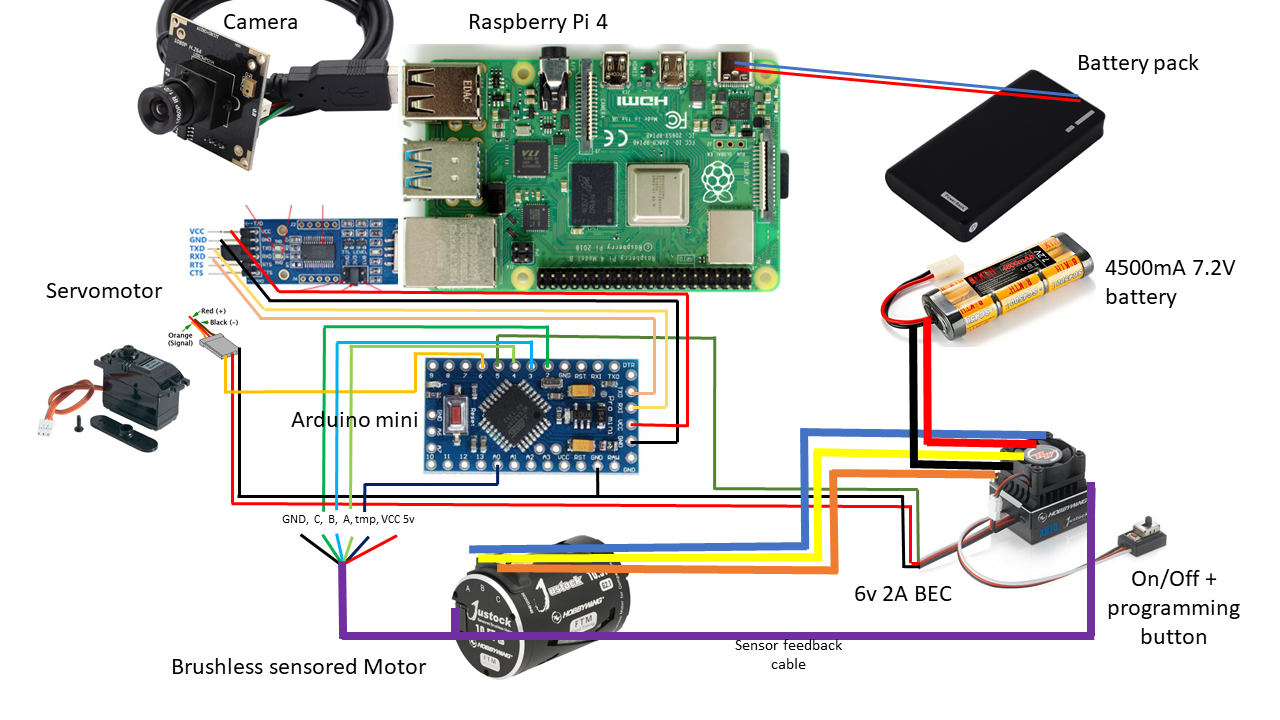
\includegraphics[width=27cm]{schema.png}}


\subsection{Software}
As you understood, our work will be focused more on the software side.
Our project will be written mostly in Python, with a bit of JS and arduino code.
We will divide the project into 3 big parts:
\begin{itemize}
\item The backend. This is where most of our efforts will be focused, this part includes every key programs all the way from the data gathering to the model training and testing.

The first part we will developp is the code responsible for the communication between the RaspberryPi and the Arduino, this code will enable us to drive the motor and servo motor by calling some simple functions. This program will also later be used to fetch the speed of the car transmitted by the arduino to the RaspberryPi.
Then, we will need to find a way to control the car manually, for example using a controller. The values of every axis and buttons on the controller
\item The Telemetry website. This part will give us the ability to see in real time the last predictions of our model and plot some data found usefull like the speed of the car.
\item The presentation website. This website will evolve with the time, tracking our latest acheivements and demonstration videos.
\end{itemize}

 
\subsection{Constraints}
Throughout the project, we will have to keep in mind some constraints.
Our biggest constraint will be the compute power. We need all of the inference of the model to be executed on the RaspberryPi, this means that we will have to be really carefull of the performance of our code. How fast our main control loop is will determine the reactivity of our car. Our usb camera can capture up to 30 images per seconds, our main control loop should ideally match 30 iterations per seconds. For example, if the car is going at 1 meter per seconds and our control loop is running at 10hz, the distance the car travels between each iteration is 10cm. Now if you are going 5 times faster with the same control loop, you now have 50cm between each decision, this is huge for such a small car ! The part that will likely take the most time will be the inference, we will need to keep track of the ratio between performance and accuracy of our models.
Regarding the accuracy of our models, we will need sufficient accuracy and generalization to be able to complete multiple laps. If the generalization is not high enough, small changes in the lightning or changes in the background will affect the prediction of our model.
On the safety part, we have to keep in mind that we are driving a powerfull car, a wrong motor command can lead us right into the wall and break the car. Prior to deploy and test our code on a real track, we will need to carefully test our code to avoid such a disaster.
\newpage

% sout : 7 / 03 & 25 / 04 & 06 / 06
\section {Planning}
\subsection {Race}

\begin{tabular}{|l|c|c|c|c|c|c|} 
\hline
\begin{tabular}[c]{@{}l@{}}\\Tasks\end{tabular} & Race 1 & Race 2 & Race 3 & Race 4 & Race 5 & Race 6  \\ 
\hline
Code controlled motors and servo                & 75\%   & 100\%  &        &        &        &         \\ 
\hline
Drive the car with a controller                 & 25\%   & 100\%   &        &        &        &         \\ 
\hline
Data collection                                 &        & 50\%   & 100\%  &        &        &         \\ 
\hline
Telemetry website                               &        & 25\%   & 100\%  &        &        &         \\ 
\hline
Data processing and augmentation                &        &        & 50\%   & 75\%   & 100\%  &         \\ 
\hline
Basic Convolutional neural network              &        &        & 25\%   & 50\%   & 100\%  &         \\ 
\hline
\begin{tabular}[c]{@{}l@{}}Advanced \\models and optional objectives\end{tabular} &        &        &        &        &        & 50\%    \\
\hline
\end{tabular}

\subsection {Presentations}

\begin{tabular}{|l|c|c|c|} 
\hline
Tasks                                                                             & 1st presentation & 2nd Presentation & Final resentation  \\ 
\hline
Code controlled motors and servo                                                  & 100\%              &                &                    \\ 
\hline
Drive the car with a controller                                                   & 100\%              & ~              &                    \\ 
\hline
Data collection                                                                   & 75\%               & 100\%          &                    \\ 
\hline
Telemetry website                                                                 & 25\%               & 100\%          &                    \\ 
\hline
Data processing and augmentation                                                  &                    & 75\%           & 100\%              \\ 
\hline
Basic Convolutional neural network                                                &                    & 50\%           & 100\%              \\ 
\hline
\begin{tabular}[c]{@{}l@{}}Advanced \\models and optional objectives\end{tabular} &                    &                & 50\%               \\
\hline
\end{tabular}


\section {Task allocation}

\begin{tabular}{|l|c|c|c|c|} 
\hline
Tasks                        & Mickael B. & Maxime G. & Alexandre G. & Maxime E.  \\ 
\hline
Low level car control        &            & x         & x            &            \\ 
\hline
Driving with a controller    &            & x         & x            &            \\ 
\hline
Data storage and handling    & x          & x         & x            & x          \\ 
\hline
Telemetry website            & x          &           &              & x          \\ 
\hline
Presentation website         & x          &           &              & x          \\ 
\hline
Convolutional neural network & x          & x         & x            & x          \\ 
\hline
Main control loop            &            & x         & x            & x          \\
\hline
\end{tabular}


% Maybe write later
\section {Conclusion}
All in all our project is not an easy one, as you might have realized, it will take a lot of work and learning to make it work. But we are motivated to learn, listen and work. Our goal is not to revolutionise the automobile industry but juste to make something that we enjoy and get a first glance into what AI and self driving cars are all about. 
... to finish


\end{document}
